\subsubsection{O que é diagrama de definição de blocos}

O diagrama de definições de bloco é baseado no diagrama de classes da UML com o adicional de algumas restrições e extensões definidas dentro da SysML. Sendo o diagrama mais usado dentro dessa. Sua função é modelar os aspectos estruturais, através de blocos, de um sistema, mostrando os elementos físicos, relacionamentos, fluxos e hierarquias.

\subsubsection{Estrutura dos diagramas de definição de blocos}

Com a proposta de mostrar diferentes elementos do fluxo e suas relações a figura abaixo mostra o diagrama de definição de blocos de uma ACME câmera, com os símbolos mais comuns do diagrama de blocos.


\begin{figure}[h]
\centering
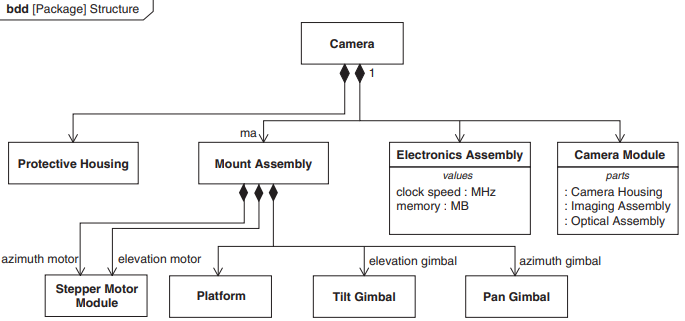
\includegraphics[width=\textwidth,height=\textheight,keepaspectratio]{figures/diagrama de blocos.PNG}
\caption{?????????????????????????}
\label{fig:block_diagram}
\end{figure}

\paragraph{}
 \textbf{Elementos físicos} 
 
 
Os elementos físicos são graficamente representados por blocos. Eles podem ser hardwares, softwares, pessoas ou qualquer outra entidade lógica ou conceitual. O nome do bloco aparece em seu topo em negrito, enquanto as outras propriedades tem seus compartimentos abaixo em letra minúscula, itálico e espaço entre as palavras. Essas propriedades podem ser de três diferentes tipos. Uma delas é propriedade de parte, que decompõem o bloco nos elementos que os constituem. Outra é a propriedade de referência, que referencia partes de outro bloco indicando em que partes o blocos conectados se relacionam. Por fim, pode-se ter também a propriedade de valor, responsável por descrever as características quantificáveis do bloco.

\paragraph{}
 \textbf{Relacionamento entre blocos} 
 
O relacionamento entre blocos indica como os blocos se relacionam, de maneira geral ele é representado com uma linha simples com elementos nas pontas, que irá indicar qual a relação exata entre eles. Existem quatro tipos diferentes de relação que podem ser representados no diagrama de blocos. 

A conexão de composição é representada graficamente por um losango preenchido conectado em um bloco maior com um traço embaixo ligando a outros blocos, é utilizado para indicar que o bloco maior possui outros elementos definindo assim uma propriedade de parte no bloco maior. Existe a possibilidade de se colocar uma seta na outra parte, neste caso faz alusão a alguma propriedade referência. 

A conexão de referência é representada graficamente por um losangolo vazio em uma ponta ligado por uma seta a outros elementos. Ela é utilizada para indicar que um bloco referencia o outro, quando existe uma referencia apenas de um lado da relação é utilizada uma seta no bloco que contém a propriedade de referência, já se ambos blocos se referenciam entre si não são utilizadas setas.

A conexão por associação pode ser utilizada tanto para definir como blocos podem estar validamente conectados quanto para detalhar essa conexão, podendo ter sua própria estrutura interna e diferentes camadas. Ela é representada por uma linha entre os dois blocos a serem conectados, ligados a uma linha tracejada partindo do meio da linha principal que leva a um terceiro bloco, responsável por detalhar a conexão. 

A conexão generalizada, indica a relação entre um bloco geral e um específico. Ela é representada graficamente por uma seta de cabeça fechada ligada ao bloco geral e uma linha simples ao bloco específico.

\paragraph{}
 \textbf{Fluxo entre os blocos} 
 
Para modelar o fluxo entre os blocos, são necessários três elementos; a porta, que representa os ponto de troca. o  fluxo de item, que define a direção que às trocas se dão e a propriedade de fluxo, irá indicar qual é a propriedade e se ela irá sair ou entrar do elemento. Assim como de conexões, existem diferentes tipos de portas. Podendo ser uma porta completa, com entrada e saída para dentro do diagrama, uma porta de proxy, onde só a entrada ou a saída estão diretamente ligadas ao diagrama ou uma porta de proxy com interface, que, onde o usuário insere a entrada no sistema. As duas primeiras são representadas por quadrados nas laterais do bloco e o último por alavancas com bolas ou semi-bolas.

    \subsubsection{Aplicação}
    
Uma aplicação para o diagrama de blocos é o uso em sistemas embarcados de tempo real. Um sistema embarcado é um sistema embutido em um hardware com um propósito de aplicação responsável por controlar e executar as funções deste hardware. Quando se trata de um sistema de tempo real, adiciona-se um grau a mais de dificuldade devido a aspectos específicos desses sistemas como mobilidade, segurança ou restrição de tempo real. Com a união de hardware e software, existe uma interação contínua com o ambiente por meio de sensores e atuadores. 

O sistema de airbag conversa com o controle de comunicação, que por sua vez extrai informações do controle de velocidade cuja a fonte são o relógio e o sensor de velocidade e do controle de peso. Estando conectado também ao controle de dashboard, responsável por comunicar o mal funcionamento do airbag. Além disso, ele recebe informações sensor e transmite para o controle de sistema do atuador que por sua vez, repassa para o atuador do airbag. Todos esses elementos e comunicações podem ser simplificados através de um digrama de definição de blocos.
